\documentclass[border = 1cm]{standalone}

\usepackage{tikz}
\usetikzlibrary{mindmap,trees}
\usepackage{verbatim}

\begin{document}
\pagestyle{empty}

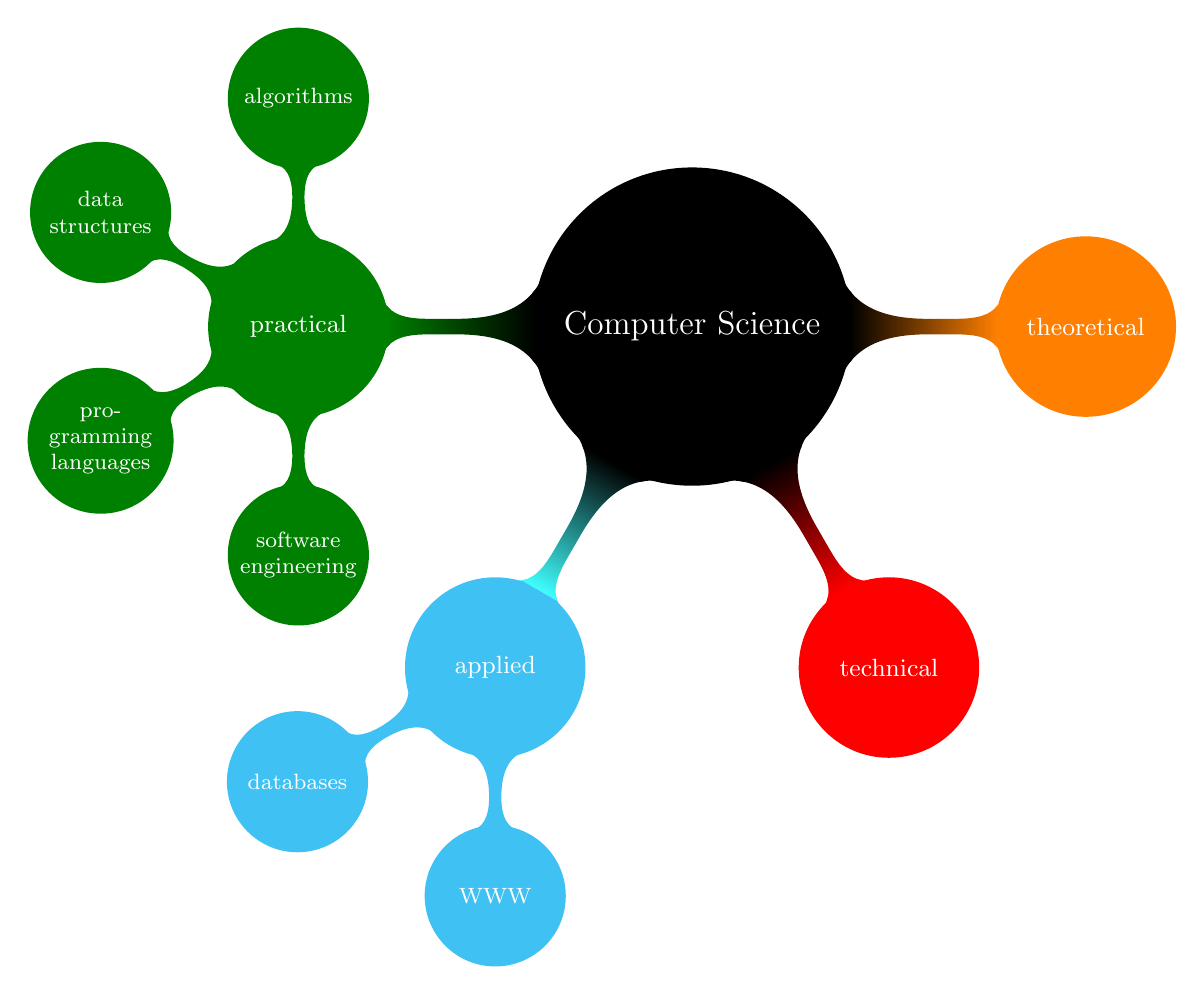
\begin{tikzpicture}[rotate=-90]
  \path[mindmap,concept color=black,text=white, grow cyclic]
    node[concept] {Computer Science}
    child[concept color=green!50!black]
    {
        node[concept] {practical}
        child { node[concept] {algorithms} }
        child { node[concept] {data structures} }
        child { node[concept] {pro\-gramming languages} }
        child { node[concept] {software engineer\-ing} }
    }  
    child[concept color=cyan!75]
    {
        node[concept] {applied}
        child { node[concept] {databases} }
        child { node[concept] {WWW} }
    }
    child[concept color=red] { node[concept] {technical} }
    child[concept color=orange] { node[concept] {theoretical} };
\end{tikzpicture}
\end{document}